% Dokumentklasse
% --------------
\documentclass[12pt,naustrian,a4widepaper]{scrartcl}   
% article style
%   - 11pt Schriftgroesse
%   - new austrian (neue Rechtschreibung)
%   - Papierformat A4
%   - pdf-hyperlinks

%****************In her all definitions are listed*********************
\usepackage[ngerman]{babel} 					% wegen deutschen Umlauten
\usepackage[utf8]{inputenc}
\usepackage{amsmath}
\usepackage[usenames,dvipsnames]{xcolor}
\usepackage{pdfpages}
\usepackage{lastpage} 							% Required to determine the last page for the footer
%\usepackage{amsmath}
\usepackage{float}
\usepackage{hyperref}
\usepackage{listings}
\usepackage{graphicx}							% Einbinden von Bildern
%\usepackage{multicol} 							% Spalten
%\usepackage{textcomp} 							% spitze klammern
%\usepackage{hyperref}  						% hyperlinks
\usepackage[absolute]{textpos}
\usepackage{xcolor}
\usepackage{tabularx}
\usepackage{tcolorbox}
\usepackage{enumitem}
\usepackage{fancyhdr}   % für Kopf- und Fusszeilen
%*************************************************************************
\pagestyle{fancy} 						% Wird für den Header gebraucht

% Seitenspiegel
% -------------

\typearea{8}	% Festlegung des Seitenspiegels gem. Koma. 4..groß, 9..klein


% Kopfzeile
% ---------
\lhead{{\footnotesize{\docauthor, \doccoauthor}}}   %  (links)
\chead{{\footnotesize{Systemdokumentation - \docproject}}} %  (mitte)
\rhead{{\footnotesize{Seite \thepage}}}      %  (rechts)

% Fusszeile
% ---------
\lfoot{}  % links
\cfoot{}  % mitte 
\rfoot{}  % rechts

% Absatzformatierung
% ------------------
\setlength{\parindent}{0cm}   % Einrückung der 1. Zeile jedes Absatzes
\setlength{\parskip}{10pt}    % Abstand zwischen den Absätzen

\selectlanguage{naustrian}   % oder "american" für engl. Texte

% Titelblatt
% ----------
\newcommand{\hgbtitle}{
\title {\vspace{1cm}
	
\includegraphics[width=8cm]{./Images/FhOOeLogoOkt2009_HSD_Rot_pastell}\\
	\vspace{2cm}
	{\textbf{Systemdokumentation\\Projekt \docproject}}\\
	\vspace{5mm}
	{\small{Version 1.0}}\\
	\vspace{5mm}
}

\author{\small{\docauthor, \doccoauthor}}
\date  {\small{Hagenberg, \today}}
\maketitle
}

%****************** self defined commands ***************************
%include a pseudocode file
%usage: \pseudocode{Title}{path_to_your_file/filename} (relative to Übung root folder)
\newcommand{\pseudocode}[2]{
\begin{itemize}
\item[]\lstinputlisting[caption="#1",label="#1", style=pseudocodeStyle]{../#2}
\end{itemize}
}

% Include Linux terminal output
% Usage: \linuxoutput{Title}{path_to_your_file/filename}
\newcommand{\linuxoutput}[2]{
	\begin{itemize}
		\item[]\lstinputlisting[
		caption="#1",
		label="#1",
		style=linuxStyle
		]{../#2}
	\end{itemize}
}

% include an ARM Assembly source file
% usage: \armasm{path_to_your_file/filename}
%        (relative to Übung root folder)
\newcommand{\armasm}[1]{
	\begin{itemize}
		\item[]\lstinputlisting[
		caption="#1.s",
		label="#1.s",
		style=armasm
		]{../#1.s}
	\end{itemize}
}

% Usage: \bashscript{Title}{path_to_script}
\newcommand{\bashscript}[2]{
	\begin{itemize}
		\item[]\lstinputlisting[caption="#1",label="#1",style=bashStyle]{../#2}
	\end{itemize}
}

%include a .cpp source file
%usage: \cpp{path_to_your_file/filename}(relative to Übung root folder)
\newcommand{\cpp}[1]{
\begin{itemize}
\item[]\lstinputlisting[caption="#1.cpp",label="#1.cpp", style=customcpp]{../#1.cpp}
\end{itemize}
}

%include a .c source file
%usage: \cfile{path_to_your_file/filename}(relative to Übung root folder)
\newcommand{\cfile}[1]{
	\begin{itemize}
		\item[]\lstinputlisting[caption="#1.c",label="#1.c", style=customcpp]{../#1.c}
	\end{itemize}
}

%include a .h source file
%usage: \h{path_to_your_file/filename} (relative to Übung root folder)
\newcommand{\h}[1]{
\begin{itemize}
\item[]\lstinputlisting[caption="#1.h",label="#1.h", style=customcpp]{../#1.h}
\end{itemize}
}

%include a module (.cpp and .h)
%usage: \cppmodule{path_to_your_file/filename} (relative to Übung root folder)
\newcommand{\cppmodule}[1]{
\begin{itemize}
\item[]\lstinputlisting[caption=#1.h,label=#1.h, style=customcpp]{../#1.h}
\item[]\lstinputlisting[caption=#1.cpp,label=#1.cpp, style=customcpp]{../#1.cpp}
\end{itemize}
}

%include a code snippet
%usage: \snippet{path_to_your_file/filename}{startline}{endline} (relative to Übung root folder)
\newcommand{\snippet}[3]{
\begin{itemize}
\item[]\lstinputlisting[caption=#1.cpp,label=#1.cpp, style=customcpp, firstline=#2,lastline=#3]{../#1.cpp}
\end{itemize}
}

%include a test-output file 
%usage: \testoutput{path_to_your_file/filename} (relative to Übung root folder)
\newcommand{\testoutput}[1]{
\begin{itemize}
\item[]\lstinputlisting[caption=#1]{../#1.txt}
\end{itemize}
}

%include a figure 
%usage: \fig{path_to_your_file/filename}{width}{caption text} (relative to Übung root folder)
%width between 0.0 - 1.0 -> correspond with textwidth
\newcommand{\fig}[3]{
\begin{figure}[H]
\centering
\includegraphics[width=#2\textwidth]{../#1}
\caption{#3}
\label{fig:fig1}
\end{figure}
}

%include a flowchart
%usage: \flow{path_to_your_file/filename} (relative to Übung root folder)
\newcommand{\flow}[3]{
\begin{figure}[H]
\centering
\includegraphics[width=0.5\textwidth]{../#1.png}
\caption{Flussdiagramm #1}
\label{fig:fig1}
\end{figure}
}


\lstset{
   literate      = 
      {á}{{\'a}}1  {é}{{\'e}}1  {í}{{\'i}}1 {ó}{{\'o}}1  {ú}{{\'u}}1
      {Á}{{\'A}}1  {É}{{\'E}}1  {Í}{{\'I}}1 {Ó}{{\'O}}1  {Ú}{{\'U}}1
      {à}{{\`a}}1  {è}{{\`e}}1  {ì}{{\`i}}1 {ò}{{\`o}}1  {ù}{{\`u}}1
      {À}{{\`A}}1  {È}{{\`E}}1  {Ì}{{\`I}}1 {Ò}{{\`O}}1  {Ù}{{\`U}}1
      {ä}{{\"a}}1  {ë}{{\"e}}1  {ï}{{\"i}}1 {ö}{{\"o}}1  {ü}{{\"u}}1
      {Ä}{{\"A}}1  {Ë}{{\"E}}1  {Ï}{{\"I}}1 {Ö}{{\"O}}1  {Ü}{{\"U}}1
      {â}{{\^a}}1  {ê}{{\^e}}1  {î}{{\^i}}1 {ô}{{\^o}}1  {û}{{\^u}}1
      {Â}{{\^A}}1  {Ê}{{\^E}}1  {Î}{{\^I}}1 {Ô}{{\^O}}1  {Û}{{\^U}}1
      {œ}{{\oe}}1  {Œ}{{\OE}}1  {æ}{{\ae}}1 {Æ}{{\AE}}1  {ß}{{\ss}}1
      {ẞ}{{\SS}}1  {ç}{{\c{c}}}1 {Ç}{{\c{C}}}1 {ø}{{\o}}1  {Ø}{{\O}}1
      {å}{{\aa}}1  {Å}{{\AA}}1  {ã}{{\~a}}1  {õ}{{\~o}}1 {Ã}{{\~A}}1
      {Õ}{{\~O}}1  {ñ}{{\~n}}1  {Ñ}{{\~N}}1  {¿}{{?`}}1  {¡}{{!`}}1
      {„}{\quotedblbase}1 {“}{\textquotedblleft}1 {–}{$-$}1
      {°}{{\textdegree}}1 {º}{{\textordmasculine}}1 {ª}{{\textordfeminine}}1
      {£}{{\pounds}}1  {©}{{\copyright}}1  {®}{{\textregistered}}1
      {«}{{\guillemotleft}}1  {»}{{\guillemotright}}1  {Ð}{{\DH}}1  {ð}{{\dh}}1
      {Ý}{{\'Y}}1    {ý}{{\'y}}1    {Þ}{{\TH}}1    {þ}{{\th}}1    {Ă}{{\u{A}}}1
      {ă}{{\u{a}}}1  {Ą}{{\k{A}}}1  {ą}{{\k{a}}}1  {Ć}{{\'C}}1    {ć}{{\'c}}1
      {Č}{{\v{C}}}1  {č}{{\v{c}}}1  {Ď}{{\v{D}}}1  {ď}{{\v{d}}}1  {Đ}{{\DJ}}1
      {đ}{{\dj}}1    {Ė}{{\.{E}}}1  {ė}{{\.{e}}}1  {Ę}{{\k{E}}}1  {ę}{{\k{e}}}1
      {Ě}{{\v{E}}}1  {ě}{{\v{e}}}1  {Ğ}{{\u{G}}}1  {ğ}{{\u{g}}}1  {Ĩ}{{\~I}}1
      {ĩ}{{\~\i}}1   {Į}{{\k{I}}}1  {į}{{\k{i}}}1  {İ}{{\.{I}}}1  {ı}{{\i}}1
      {Ĺ}{{\'L}}1    {ĺ}{{\'l}}1    {Ľ}{{\v{L}}}1  {ľ}{{\v{l}}}1  {Ł}{{\L{}}}1
      {ł}{{\l{}}}1   {Ń}{{\'N}}1    {ń}{{\'n}}1    {Ň}{{\v{N}}}1  {ň}{{\v{n}}}1
      {Ő}{{\H{O}}}1  {ő}{{\H{o}}}1  {Ŕ}{{\'{R}}}1  {ŕ}{{\'{r}}}1  {Ř}{{\v{R}}}1
      {ř}{{\v{r}}}1  {Ś}{{\'S}}1    {ś}{{\'s}}1    {Ş}{{\c{S}}}1  {ş}{{\c{s}}}1
      {Š}{{\v{S}}}1  {š}{{\v{s}}}1  {Ť}{{\v{T}}}1  {ť}{{\v{t}}}1  {Ũ}{{\~U}}1
      {ũ}{{\~u}}1    {Ū}{{\={U}}}1  {ū}{{\={u}}}1  {Ů}{{\r{U}}}1  {ů}{{\r{u}}}1
      {Ű}{{\H{U}}}1  {ű}{{\H{u}}}1  {Ų}{{\k{U}}}1  {ų}{{\k{u}}}1  {Ź}{{\'Z}}1
      {ź}{{\'z}}1    {Ż}{{\.Z}}1    {ż}{{\.z}}1    {Ž}{{\v{Z}}}1  {ž}{{\v{z}}}1
      {¢}{{$\not\subset$}}1 {§}{{\S}}1 {¥}{{\textyen}}1   ,
   inputencoding=ansinew,
   extendedchars=true,
   basicstyle=\scriptsize\ttfamily,
   numberstyle=\scriptsize,
   breaklines=true,
   tabsize=4,
   numbersep=5pt
}

\lstdefinestyle{customcpp}{
   language=C++,
   frame=single,
   %backgroundcolor=\color{mygray},
   numbers=left,
   keywordstyle=\color{blue}\bfseries,
   stringstyle=\color{BrickRed}\ttfamily,
   commentstyle=\color{OliveGreen}\ttfamily,
   showspaces=false,
   showstringspaces=false,
   showtabs=false,
   xleftmargin=5px,    
}

\usepackage[T1]{fontenc}
\usepackage[utf8]{inputenc}
\usepackage[dvipsnames]{xcolor}
\usepackage{listings}
\usepackage{lmodern}

% --------------------------------------------------------------------------
% ARM Assembly language definition
% --------------------------------------------------------------------------
\lstdefinelanguage{ARMASM}{
	morekeywords=[1]{
		AREA,ALIGN,ALIGNR,ATTR,EXPORT,IMPORT,PROC,ENDP,END,
		PRESERVE8,THUMB,CODE,DATA,READONLY,READWRITE,NOINIT,
		DCD,DW,DCW,DCB,SPACE,EQU
	},
	morekeywords=[2]{
		LDR,STR,LDM,STM,LDMIA,STMIA,
		PUSH,POP,MOV,MVN,
		ADD,ADC,SUB,SBC,MUL,MLS,MLA,
		AND,ORR,EOR,BIC,
		CMP,CMN,TST,TEQ,
		B,BL,BX,BLX,
		BEQ,BNE,BCS,BHS,BCC,BLO,
		BMI,BPL,BVS,BVC,BHI,BLS,
		BGE,BLT,BGT,BLE
	},
	morekeywords=[3]{
		R0,R1,R2,R3,R4,R5,R6,R7,
		R8,R9,R10,R11,R12,SP,LR,PC,
		APSR,CPSR
	},
	morekeywords=[4]{
		DCD,DW,DCW,DCB,SPACE,EQU
	},
	sensitive=false,
	morecomment=[l]{;},
	morestring=[b]"
}

% --------------------------------------------------------------------------
% ARM Assembly style
% --------------------------------------------------------------------------
\definecolor{armblue}{RGB}{0,70,140}
\definecolor{armgreen}{RGB}{0,120,70}
\definecolor{armred}{RGB}{170,40,40}
\definecolor{armgray}{RGB}{100,100,100}
\definecolor{armpurple}{RGB}{110,50,140}

\lstdefinestyle{armasm}{
	language=ARMASM,
	basicstyle=\ttfamily\small,
	columns=fullflexible,
	keepspaces=true,
	keywordstyle=[1]\color{armblue}\bfseries,
	keywordstyle=[2]\color{armred}\bfseries,
	keywordstyle=[3]\color{armpurple},
	keywordstyle=[4]\color{armgreen}\bfseries,
	commentstyle=\color{armgray}\itshape,
	stringstyle=\color{armgreen},
	numbers=left,
	numberstyle=\tiny\color{armgray},
	numbersep=8pt,
	frame=single,
	rulecolor=\color{black!25},
	framesep=5pt,
	breaklines=true,
	breakatwhitespace=false,
	showstringspaces=false,
	tabsize=8,	
	captionpos=b
}


\lstdefinelanguage{linux}{
	sensitive=true,
	morekeywords={cd,ls,cat,touch,rm,mkdir,rmdir,cp,mv,pwd,echo,grep,find,chmod,chown,tar,clear,exit},
	morestring=[b]"
}

\lstdefinestyle{linuxStyle}{
	language=linux,
	frame=single,
	numbers=none,
	basicstyle=\ttfamily\footnotesize\color{black},
	keywordstyle=\color{Blue}\bfseries,
	stringstyle=\color{BrickRed},
	emph={tlech@DESKTOP,MPJVO86},
	emphstyle=\color{Green}\bfseries,
	showspaces=false,
	showstringspaces=false,
	showtabs=false,
	breaklines=true,
	breakatwhitespace=false,
	xleftmargin=5px,
	literate=
	{_}{{\_}}1
	{ä}{{\"a}}1
	{ö}{{\"o}}1
	{ü}{{\"u}}1
	{Ä}{{\"A}}1
	{Ö}{{\"O}}1
	{Ü}{{\"U}}1
	{ß}{{\ss}}1
}

\lstdefinelanguage{bash}{
	sensitive=true,
	morekeywords={
		if,then,else,elif,fi,
		for,while,until,in,
		do,done,
		case,esac,
		function,
		select,
		time,
		coproc,
		return,
		local,
		declare,
		readonly,
		export,
		unset,
		shift,
		getopts,
		source,
		echo,
		printf,
		read,
		cd,
		pwd,
		test,
		true,
		false,
		type,
		command,
		builtin,
		eval,
		exec,
		exit,
		let
	},
	morestring=[b]",
	morestring=[b]',
	morecomment=[l]\#
}

\lstdefinestyle{bashStyle}{
	language=bash,
	frame=single,
	numbers=left,
	numberstyle=\tiny\color{gray},
	basicstyle=\ttfamily\small\color{black},
	keywordstyle=\color{Blue}\bfseries,
	stringstyle=\color{BrickRed},
	commentstyle=\color{OliveGreen},
	showspaces=false,
	showstringspaces=false,
	showtabs=false,
	breaklines=true,
	breakatwhitespace=false,
	keepspaces=true,
	columns=fullflexible,
	xleftmargin=5px
}


\lstdefinelanguage{pseudocode}{
  morekeywords={if, then, else, elseif, case, of, while, do, repeat, until, for, to, by, end, algorithm, const, static, bool, int, char, double, string, real, array, param, local, modulo, halt, return, not, size\_t, and, or, xor},
  sensitive=true,
  morecomment=[l]{//},
  morestring=[b]"
}

% Define a style for pseudocode listings
\lstdefinestyle{pseudocodeStyle}{
  language=pseudocode,
   frame=none,
   numbers=none,
   keywordstyle=\underline,
   stringstyle=\color{BrickRed}\ttfamily,
   commentstyle=\color{OliveGreen}\ttfamily,
   showspaces=false,
   showstringspaces=false,
   showtabs=false,
   xleftmargin=5px,
   literate={!=}{{$\neq$}}1
   			{=}{{$\leftarrow$}}1 
   			{==}{{$==$}}1
   			{<=}{{$\leq$}}1
   			{>=}{{$\geq$}}1
   			{°}{{$\downarrow$}}1 
			{\#}{{$\updownarrow$}}1 
   			{^}{{$\uparrow$}}1 
   			{ö}{{\"o}}1
           	{ä}{{\"a}}1
           	{ü}{{\"u}}1
           	{ß}{{\ss}}1
           	{é}{{\'e}}1
}


% For function descriptions
% ---------- Parameter ----------
\newcommand{\param}[1]{\item #1}

% ---------- Function Command ----------
% #1 function signature
% #2 parameter items (\param{...})
% #3 description
\newcommand{\func}[3]{%
\begin{tcolorbox}[
    colback=white,          % white background for main box
    colframe=black!50,      % subtle border
    colbacktitle=white,     % white background for the title/header
    coltitle=black,         % black text for the title
    boxrule=0.6pt,          % border thickness
    arc=1mm,                % rounded corners
    left=6pt, right=6pt, top=4pt, bottom=4pt,
    fonttitle=\ttfamily\bfseries,
    title={#1}              % function signature in header
]
% Only show parameters if provided
\ifx&#2&%
  % do nothing
\else
\textbf{Parameter}%
\begin{itemize}[topsep=0pt, partopsep=0pt, parsep=0pt, itemsep=0pt, leftmargin=*]
#2
\end{itemize}
\fi

\textbf{Beschreibung} #3

\end{tcolorbox}%
\vspace{2pt} % minimal spacing after box
}

%*************************Dokumenteninfos*******************************
\newcommand{\docproject}{Musik-Player}			% Projektname
\newcommand{\docsubject}{Software Design Patterns}	% Fach
\newcommand{\docsubjectshort}{SDP3}					% Fach-Kürzl
\newcommand{\docexercise}{Übung 6}					% Übungstitel
\newcommand{\docauthor}{T. Lechner}					% Name
\newcommand{\doccoauthor}{P. Ackermann}				% Name
\newcommand{\docauthornumber}{S2510306017}			% Martrikelnummer
\newcommand{\doccoauthornumber}{S2510306001}		% Martrikelnummer
\newcommand{\docauthoremail}{s2510306017@students.fh-hagenberg.at}
\newcommand{\doccoauthoremail}{s2510306001@students.fh-hagenberg.at}
\newcommand{\docdate}{\date}						% Datum	
\newcommand{\docsemester}{Wintersemester 2026/2027}	% Semester
%%%%%%%%%%%%%%%%%%%%%%%%%%%%%%%%%%%%%%%%%%%%%%%%%%%%%%%%%%%%%

\begin{document}


%%%%%%%%%%%%%%%%%%%%%%%%%%%%%%% Angabe.pdf %%%%%%%%%%%%%%%%%%%%%%%%%%%%%%%
\begin{textblock*}{80mm}(43mm,70mm)
	\docauthor, \doccoauthor
\end{textblock*}
\begin{textblock*}{80mm}(44mm,84mm)
	\docauthornumber, \doccoauthornumber
\end{textblock*}
\begin{textblock*}{40mm}(60mm,99mm)
	1 					% Übungsgruppe
\end{textblock*}
\begin{textblock*}{40mm}(155mm,70mm)
	12					% Stunden
\end{textblock*}

% Inkludieren der Angabe
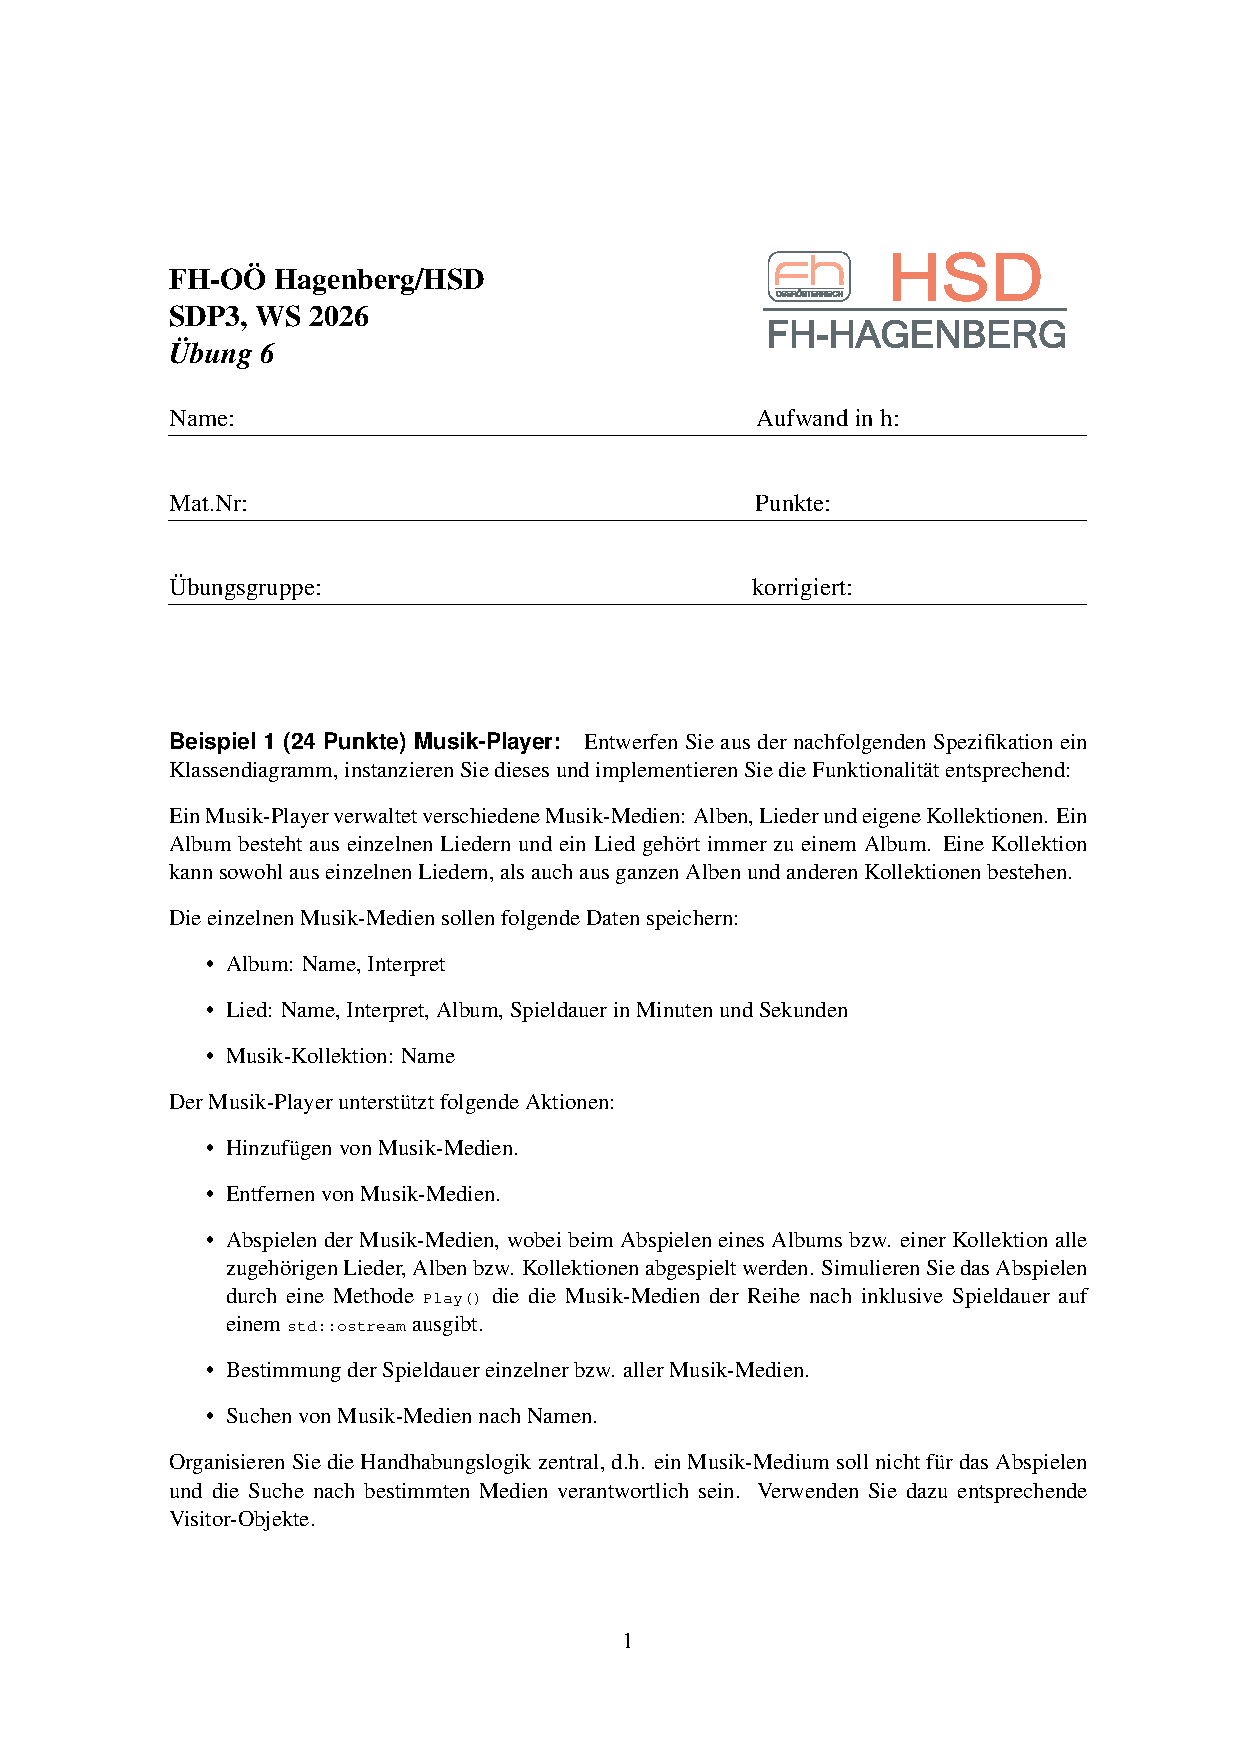
\includepdf[pages=-]{Angabe.pdf}
\newpage
\hgbtitle
\newpage


%%%%%%%%%%%%%%%%%%%%%%%%%%%%%%% Inhaltsverzeichnis %%%%%%%%%%%%%%%%%%%%%%%%

\tableofcontents
\newpage

%%%%%%%%%%%%%%%%%%%%%%%%%%%%%%% Ausarbeitung %%%%%%%%%%%%%%%%%%%%%%%%%%%%%%

\section{Organisatorisches}

\subsection{Team}
\begin{itemize}
	\item \docauthor, Matr.-Nr.: \docauthornumber, E-Mail: \docauthoremail	
	\item \doccoauthor, Matr.-Nr.: \doccoauthornumber, E-Mail: \doccoauthoremail
\end{itemize}

\subsection{Aufteilung der Verantwortlichkeitsbereiche}
\begin{itemize}
	\item \docauthor
	\begin{itemize}
		\item Implementierung und Unit-Test:
		\begin{itemize}
			\item Object
			\item SearchVisitor
			\item PrintVisitor
			\item MusicPlayer
			\item PlaylistFactory
			\item SongRepository
		\end{itemize}
	\end{itemize}
	\item \doccoauthor
	\begin{itemize}
		\item Implementierung und Unit-Test:
		\begin{itemize}
			\item IPlaylistVisitor
			\item DurationVisitor
			\item PlaylistElement
			\item Song
			\item Album
			\item Collection
		\end{itemize}
	\end{itemize}	
\end{itemize}

\subsection{Aufwand}

\begin{itemize}
	\item \docauthor: geschätzt 12 Ph / tatsächlich 0 Ph
	\item \doccoauthor: geschätzt 12 Ph / tatsächlich 0 Ph
\end{itemize}

\section{Anforderungsdefinition (Systemspezifikation)}
 
\section{Systementwurf}

\subsection{Klassendiagramm}
\fig{Systemdoku/Images/MusicPlayer.png}{1.2}{Klassendiagramm \docproject}

\subsection{Designentscheidungen}

Als Basisklasse aller Basisklassen dient wieder die \textbf{Object} Klasse.\\

Für das Speichern der Musik-Medien wird ein \textbf{Composite}-Pattern verwendet. \textbf{PlaylistElement} ist dabei die gemeinsame abstrakte Basisklasse. Da jedes Medium einen Namen besitzen muss, wird dieser auch in \textbf{PlaylistElement} implementiert.\\

Alle \textbf{PlaylistElement}e werden mit der \textbf{PlaylistFactory}, einer einfachen \textbf{Factory}-Klasse, erzeugt.\\

Der allgemeine Container für Musik-Medien ist eine \textbf{Collection}, in der beliebig viele \textbf{PlaylistElement} shared\_ptr gespeichert sind. Dort können beliebig neue Elemente hinzugefügt und wieder entfernt werden.\\

Ein \textbf{Album} ist insofern speziell, da es nur \textbf{Song}s speichern kann und keine anderen Musik-Medien. Ein \textbf{Song} muss immer zu einem \textbf{Album} gehören und kann nicht ohne \textbf{Album} existieren, da der Interpret über das \textbf{Album} gespeichert wird. Die Dauer in Sekunden (kann dann in die gefragten Minuten und Sekunden umgerechnet werden) und der Name des Songs werden natürlich extra gespeichert. \textbf{Song} und \textbf{Album} sind somit absichtlich fest miteinander verbunden (und sogar \textit{friend}). Beim Konstruieren eines \textbf{Song}s muss das zugehörige \textbf{Album} mitgegeben werden, in dem mit der privaten \textbf{Add}-Methode der \textbf{Song} registriert wird. Im \textbf{Song} muss auch eine Referenz auf das \textbf{Album} gespeichert werden, damit der Interpret des \textbf{Song}s ermittelt werden kann.\\ 

Würde man hier in beide Richtungen shared\_ptr verwenden, so hätte man ein Problem mit zyklischer Abhängigkeit und müsste die Verbindungen immer wieder explizit aufbrechen, sonst kommt es zu Memory-Leaks $\rightarrow$ nicht RAII-konform.\\

Deswegen wird eine der Verbindungen mittels weak\_ptr realisiert. Im \textbf{Song} kann man das nicht machen, da dann evtl. ein \textbf{Song} ohne \textbf{Album} existieren könnte, was explizit verboten ist. Wenn \textbf{Album} eine Liste aus weak\_ptr hält, dann würde ein \textbf{Song} evtl. beim Konstruieren direkt wieder aufgelöst werden, da nichts auf ihn zeigt.\\

Um dieses Problem zu lösen, gibt es ein \textbf{SongRepository}, das als Container für alle erstellten \textbf{Song}s dient. Dort werden shared\_ptr gespeichert und die \textbf{Song}s bleiben am Leben. Wenn ein \textbf{Song} entgültig gelöscht werden soll, dann muss er auch aus diesem Repository gelöscht werden.\\

\textbf{PlaylistFactory} fügt beim Erzeugen eines \textbf{Song}s den \textbf{Song} zum \textbf{SongRepository} hinzu.\\

\textbf{PlaylistFactory} und \textbf{SongRepository} sind als \textbf{Singleton}-Klassen implementiert. Das wird durch die template-Basisklasse \textbf{SingletonBase} erreicht.\\

Um Operationen auf \textbf{PlaylistElement}en durchzuführen, wird das \textbf{Visitor}-Pattern verwendet. Es gibt mehrere \textbf{IPlaylistVisitor}s, die durch die \textbf{Composite}-Struktur von den \textbf{PlaylistElement}en durchgereicht werden.\\

\textbf{PrintVisitor} gibt zum Beispiel alle gespeicherten Daten auf einem std::ostream aus.\\
\textbf{SearchVisitor} sucht nach \textbf{PlaylistElement}en mit einem gewissen \textbf{searchPattern} im Namen. Diese werden in einem internen std::vector gespeichert. Über \textbf{cbegin} und \textbf{cend} werden dem Aufrufer die Suchergebnisse zur Verfügung gestellt.\\
\textbf{DurationVisitor} summiert die Dauer aller \textbf{PlaylistElement}e auf und stellt diese zur Verfügung.\\

\textbf{MusicPlayer} ist die oberste Manager-Klasse, mit der der Client schlussendlich interagiert. Dort können mehrere \textbf{PlaylistElement}e in eine Top-Level-Liste hinzugefügt und aus dieser entfernt werden. Es gibt die Operationen \textbf{Play}, \textbf{GetDuration} und \textbf{Search}, die auf alle \textbf{PlaylistElement}e in der Top-Level-Liste angewendet werden. Dafür werden die oben beschriebenen \textbf{IPlaylistVisitor}s verwendet.\\

Das gezielte Entfernen einzelner \textbf{PlaylistElement}e weiter unten in der Struktur ist wesentlich komplizierter und muss explizit durchgeführt werden, indem das Elternelement gesucht wird und dort das zu löschende Kind-Element entfernt wird. Einen \textbf{Song} aus einem \textbf{Album} zu löschen sollte nicht funktionieren. Dafür müssen alle Links auf den Song aufgelöst werden (in \textbf{Collection}s bzw. dem \textbf{MusicPlayer}). Derselbe Song kann nämlich nicht nur in seinem \textbf{Album} vorkommen, sondern auch mittels shared\_ptr im \textbf{MusicPlayer} oder einer \textbf{Collection}. Um dieses Löschen zu implementieren, könnte z.B. ein eigener \textbf{DeletionVisitor} verwendet werden, der alle Referenzen auf einen Song sucht und diese löscht. Das wurde jedoch aus Zeitgründen und da es in der Aufgabenstellung nicht explizit gefragt ist nicht implementiert.\\


\section{Dokumentation der Komponenten (Klassen)}

Die HTML-Startdatei befindet sich im Verzeichnis \href{run:./../doxy/html/index.html}{./../doxy/html/index.html}

\section{Testprotokollierung}

\section{Quellcode}

\end{document}
%%%%%%%%%%%%%%%%%%%%%%%%%%%%%%%%%%%%%%%%%%%%%%%%%%%%%%%%%%%%%%%%%%%%%%%%%%%